%
% $Id: ch04_implementation.tex
%
%   *******************************************************************
%   * SEE THE MAIN FILE "AllegThesis.tex" FOR MORE INFORMATION.       *
%   *******************************************************************
%
\chapter{Implementation}\label{ch:implem}
% Another possible chapter title: Experimental Results

\section{Test Suite}
% Pytest
% * Why Pytest
One of the more important decisions that was encountered during the creation of Function-Fiasco was the framework that was going to be under analysis for different test suites. A test suite is a collection of test cases, but differing frameworks have different ways to structure their tests and may execute the tests using different testing strategies. Function-Fiasco is meant to determine if a function is being pseudo-tested. This means that the focus of the framework must be on unit testing. Unit testing is the process of testing different modules of the system in isolation~\cite{friedman_voas_1995}. A unit test in the case for Python would be a test that looks to a function and determines its behaviors based on a series of different inputs. Lastly there need to be enough systems that use this framework so that Function-Fiasco can be tested on a multitude of open-source systems. There was a framework that fit both of the requirements for Function-Fiasco.

Pytest was the framework that was chosen for Function-Fiasco. Pytest supports a module based test suite. This is specifically what Function-Fiasco is trying to examine. It is examining if tests have been written effectively enough to observe if the test suite has high fault detection effectiveness. It is often that test suites are written on a module basis, so it is really easy to determine if a test passes or fails and specifically for which reason. Much of this ease is brought upon by the reports that Pytest generates. Pytest has a very useful interface, especially in the verbose mode. When Pytest runs outside of verbose, it produces a series of dots and Fs that are meant to represent the passing and failing tests in each file of the test suite. In verbose, Pytest gives the name of test and its file location, as well as a keyword that is meant to represent the passing or failing status of the test. The keyword will either be \texttt{PASSED} or \texttt{FAILED}. Also, if a test fails it will explain why. The explanatory nature of the report is why Pytest is becoming so popular. An example of the output using the verbose mode is shown in Listing \ref{PytestExample}. In this example, Pytest uses the root directory of \texttt{/home/user/Computer\_Science/Function-Fiasco/fake} to collect tests, which there are ten of. Once it does so, it runs the different tests that it collects using the input that the tests provide to determine if the behavior is functioning correctly. If a test fails, the line that displays the test name will result in a \texttt{FAILED} status and below the test listings another section will appear. This section is meant to help developers understand why the test failed and it does so by pointing out which part of the test resulted in the failing status. Another reason that Pytest is becoming popular is the plugins that are available for use. Pytest has a very useful feature that allows developers to create plugins that manipulate the way that Pytest runs in different ways, such as Pytest-repeat and Pytest-xdist~\cite{okken_2018}. Having a plugin based environment can be very helpful when running tests on different types of systems. There may be plugins that assist developers in one situation that will not apply to another situation. In each case a developer can write a plugin that will aid them in their case, and can supply it to other teams that may need it for the same type of test.

Pytest was crucial to the running of Function-Fiasco for a few reasons, namely the descriptive reports and the ability to create helpful plugins. The descriptive reports gave Function-Fiasco the ability to know the state of the test suite after tests had been executed. Function-Fiasco would manipulate the return of a function then execute the test suite, with the help of a user-created plugin named PytestFinder. Once the test suite had been executed, Function-Fiasco would read the descriptive output to determine if the test had resulted in a \texttt{PASSED} or \texttt{FAILED}. If the test had resulted in a \texttt{PASSED} when one of the underlying methods had been manipulated to produce a failing test case, the result indicates that the method is being pseudo-tested. It was helpful because Pytest allows the user to determine which directory to execute test cases from. Function-Fiasco is able to run from a different directory and apply its analysis on a completely different project, as long as the directory being tested is Pytest compatible.

\begin{figure}[t!]
\begin{lstlisting}[language = Python, numbers = left, frame = single, caption = Example of a Pytest Execution., label = PytestExample]
                ======= test session starts =======
platform linux -- Python 3.6.7, Pytest-4.0.2, py-1.7.0, pluggy-0.8.0 -- /usr/bin/python3
cachedir: .Pytest_cache
rootdir: /home/user/Computer_Science/Function-Fiasco/fake, inifile:
plugins: hypothesis-3.85.2, reload-0.1.0, finder-0.1.0
collected 7 items

tests/test_fake.py::test_output PASSED                   [ 14%]
tests/test_fake.py::test_search PASSED                   [ 28%]
tests/test_fake.py::test_length PASSED                   [ 42%]
tests/test_fake.py::test_addition PASSED                 [ 57%]
tests/test_fake.py::test_calculate PASSED                [ 71%]
tests/test_fake.py::test_check PASSED                    [ 85%]
tests/test_fake.py::test_size PASSED                     [100%]

                ======= 7 passed in 0.02 seconds =======
\end{lstlisting}
\end{figure}

% Pytest
%
% Function-Fiasco uses Pytest to see if the tests in the test suite pass or fail. It runs Pytest every time it applies the decorator to a method. The
%   * Most popular testing framework for the Python language
%   * Ease of creating plugins
%   * Descriptive reports after execution
% * How was it used
%   * Used to run the test suite that the tested system employs
% In the aspect of Function-Fiasco, Pytest is being used to run the tested system's test suite. It provides a very useful interface that can be used to determine which tests pass and which tests fail. Function-Fiasco reads in the verbose report which gives keywords of . It then determines if the test should have failed and if the keyword that it reads is \texttt{PASSED}, that method is pseudo-tested. Pytest also provides the ability to create plugins that aid developers in executing their test suite. It provides helpful documentation and hooks that allow developers to leverage this and create plugins that can be used in a multitude of ways. Function-Fiasco is being used in cooperation with two plugins that make it possible to perform this type of analysis. They are PytestFinder and PytestReload.


%   * Provides a report on which test specifically passed
%   * Used to determine if a test passes when it shouldn't

\section{Decorators}
% Decorators
% * What is a decorator?
A pseudo-tested method is predicated on the idea that a test will always pass regardless of the internal functionality of each method. Therefore Function-Fiasco needs a way to catch the output of a function to mask its functionality so that it can determine if it is being pseudo-tested. Python provides a way of running a function based on certain conditions. It is called a decorator.

%   * A wrapper for a function that modifies its behavior
Decorators provide a way to specify special operation modes for functions, by wrapping them in an extra layer of logic implemented as another function~\cite{lutz2013learning}. It is a very helpful piece of technology that is meant to assist in having other logic layers so that a piece of code may run the way that is intended, if the current environment allows it. An example would be only allowing a function to run if it is after a certain time of day, or if a limit has been passed. It is meant to be a runtime condition, so it will constantly go to the decorator to see how it should run. This functionality fits the needs of Function-Fiasco perfectly.

The other option was monkeypatching. Monkeypatching was a viable option. The issue is where the function would have been called. For monkeypatching, it seemed that the insertion of the functionality change would have to be made where the function call was, instead of where the function existed. This is problematic, as the main purpose of Function-Fiasco is to analyze the test suite for its fault detection effectivenes. Applying the monkeypatching decorator to the test suite may have caused other issues that may go unnoticed and make Function-Fiasco unsuccessful in finding pseudo-tested methods. That is why the decorator was chosen, so the insertion of the functionality change would occur at the source code level, leaving the test suite unchanged.

%   * Provides the ablity to change a functions output based on conditions
Decorators allow a function to be run, but may change the output if a condition is met. In Listing \ref{decoratorExample}, when the function \texttt{game\_sequence} is called, the decorator winner picks up the execution instead. Once this happens, a random number is rolled and if a certain condition is met, whether the random number is less than 50 or 50 and greater, a specific function is called. Instead of printing the print statement in \texttt{game\_sequence}, It will either print ``You have lost'' or ``You have won''. The functionality has been changed because of a condition that the system has determined.

\begin{figure}[t!]
\begin{lstlisting}[language = Python, numbers = left, frame = single, caption = Example of a decorator., label = decoratorExample]
def winner(func):
  if(randint(1, 100) < 50):
      def doFunc():
          print("You have lost")
      return doFunc
  else:
      def doFunc():
          print("You have won")
      return doFunc

@winner
def game_sequence():
  print("I will not be printed")
\end{lstlisting}
\end{figure}

% * How was it used
%   * It was written into the files of the system that is being tested
In Function-Fiasco, a decorator reference is written automatically into the system that is being tested on top of each of its functions. The purpose of this is to mark each of them with a \texttt{skipper} function. This \texttt{skipper} function is meant to collect the output of the marked functions to determine the return type. The writing of the decorator allows the functionality of the decorator to be altered across the whole system, so if one function called it in one locatiion and another called it in a different location, the outcome would be the same. This is important as there may be many functions that rely on the same function, but only one of them may be pseudo-tested. It is helpful to know if they all are so that the tests that need to be optimized may be relayed back to the user of the system. This allows Function-Fiasco to know if there is more than one test that is pseudo-testing as opposed to just the first one that calls the method. The alternative would be to run Pytest for as many tests as the method appears in and reapply the decorator every time. This would be very taxing on the resources of the system.
%   * Used to mask the output of the files
The actual output of the functions is masked and does not appear. This is so the actual return of the functions is not provided to the test suite and will not cause a test to pass when a mutation is trying to be created.
%   * Randomizes the expected output into the same type
Once the output has been caught and the type of the return has been determined, the fuzzing phase begins. A return of the same type is randomized, this is so that there is an elimination of the chance of the correct type also being provided. Fuzzing the return also helps determine the edge cases that need to be tested in greater detail.
The current version of the decorator used in Function-Fiasco can be found in Listing \ref{decoratorFF}. The conditional check in the case of this decorator is not about the type of return. The conditional check is to determine if the current function has been held under scrutiny yet. If it has then the function is simply run and the result is returned back. However, if the function's return has not been altered, then the condition passes. In this case, the return type of the function is collected and randomized, so that the fuzzing phase is completed. Once this randomization occurs, the randomized variable is returned. The next step in the analysis would be observing the returned variable in test cases that will hopefully produce a failing status, indicating that the function is not being pseudo-tested.

\begin{figure}[t!]
\begin{lstlisting}[language = Python, numbers = left, frame = single, caption = Decorator that Function-Fiasco uses., label = decoratorFF]
def skipper(func):
    functionsComplete = globs.functionsComplete
    checked = checkFunctionsComplete(func, functionsComplete)
    globs.checked = str(checked)
    if checked == True and globs.firstExe == True:
        def wrapper(*args, **kwargs):
            checkType(var, func.__name__)
            return var
        return wrapper
    elif checked == True and globs.firstExe == False:
        def doFunc(*args, **kwargs):
            var = func(*args, **kwargs)
            return checkType(var, func.__name__)
        return doFunc
    else:
        def doFunc(*args, **kwargs):
            var = func(*args, **kwargs)
            return var
        return doFunc
\end{lstlisting}
\end{figure}




\section{PytestReload}
% PytestReload
% * What is PytestReload?
During the creation of Function-Fiasco, an almost showstopper problem developed. When running Pytest from the command line, there is no issue. When running Pytest from a script, there is no issue. The issue only exists when you want to run Pytest from a script, while also changing the source code that Pytest is running. A developer can run Pytest one time, eliminate the functionality from the source code entirely, then run it again and see no change from the initial run of Pytest. Running Pytest from a script multiple times would make it remember past test status. This is because of the caching system that exists in the Python language. Since it is the same interpreter, the same Pytest memory will be maintained from the last run. This is an issue as Function-Fiasco is meant to run Pytest and see if the value passes when it should fail, but if this memory persists the tests would remain passing because of previous tests. So in reality the only tests that would have a successful analysis would be the tests that are testing the first method under scrutiny. So a Pytest plugin was created to combat this issue. It will reload all of the modules of the test suite before every Pytest run. So if there is a script that is running Pytest multiple times, the memory will not persist and every Pytest run would be as if it is the first one.

PytestReload is a Pytest plugin that allows developers to ``reload'' all of the modules that are being used in their test suite. This plugin combats the idea of test value permeance to allow mutation testing to occur on the system. The way that it works is by employing the loading that Python does as it collects different modules. PytestReload starts by comprising a list of all currently loaded modules in the current interpreter. Once it has done that, the modules are reloaded using the function found in Listing \ref{PytestReload}. This reloading function deletes every loaded module forcing Pytest to load them all again at the start of the test execution run. This would mean that if there would be a change in one of the files, the change would be present in the same interpreter.

\begin{figure}[t!]
\begin{lstlisting}[language = Python, numbers = left, frame = single, caption = PytestReload reloading function., label = PytestReload]
def reload():
    global initialModules
    for i in list(sys.modules.keys()):
        if i not in initialModules:
            del(sys.modules[i])
\end{lstlisting}
\end{figure}

% * How was it used?
The way pytestReload has been integrated into Function-Fiasco is during the run of Pytest. Function-Fiasco applies a decorator to every function, this decorator is meant to change the return for the certain function that is being evaluated currently. The issue is if the test values use test value permeance, the change in the return will not reflect during the Pytest execution and the previous test value will be used. Using PytestReload, the past test value is not remembered because all of the modules that the test suite uses are reloaded and the past test values are forgotten.


\section{PytestFinder}
% Impact analysis
% PytestFinder
% * What is PytestFinder
There may be a case where a developer has a test suite that contains numerous test cases that take up a lot of time and resources to run to completion. So if the developer makes a small change to a function, they have to execute the entire test suite to observe how much of an effect their change created. Executing only the tests that are associated with that function would almost eliminate the long runtime depending on the execution time of the tests that are being run and would limit the computer resources that are needed to execute. A Pytest plugin named PytestFinder has been created to aid this part of the testing phase.

PytestFinder is a Pytest plugin that allows users to enter a method name so that they may run only the test cases that the method is called in. For instance if there is a function \texttt{check} that is being called in three other functions, any test cases that directly uses \texttt{check} or any of its ``parent'' functions will be executed. This type of testing helps provide an impact analysis on the changes that were implemented into the system. An impact analysis is meant to determine how much of an effect a small change may have on a system as a whole~\cite{goknil2016rule}. For instance making a change in one function that supports many other functions in system would have a much larger impact than a function that is only meant to perform a calculation for itself.

% * Why was it created?
PytestFinder was created after Function-Fiasco ran into a resource problem that caused the execution to stop. Function-Fiasco runs the test suite for every method that it encounters. So if a system has an exceptionally large test suite that runs for an hour by itself, Function-fiasco could run for days and may still not finish because of the memory that is required to execute and store the pseudo-tested method information. PytestFinder fixes this issue by limiting the number of tests run. It also allows developers to run test functions that are specific to functions that they have just written. It provides a very fast way to determine how much of an effect the changes implemented have, and it informs the developer quickly if the test cases associated are still passing.

% * How it works?
PytestFinder employs a parent/child finding algorithm to create objects that can be referenced to produce the impact analysis of a change. The parent finding algorithm uses AST, or Abstract Syntax Trees, to determine if a function is being called from another. This is what will be referred to as a parent relationship. It will then follow the tree recursively to determine the parents for the newly found parents. Once this has been accomplished, every parent that has been collected during the execution of the tree is then assigned as a parent to the currently observed function. This process will continue until every function has an object created with fully processed parents. The next phase of PytestFinder is the child finding algorithm. This portion of the execution does not use AST, instead it uses the already determined parent lists. The algorithm will go through each of the parent lists of the objects and assign every parent a child that it calls. This will be referred to as a child relationship. The process of determining the children of each child is necessary because it is how the system explains what methods are being called when a test is using a specific method. This information is used to help calculate the coverage in Function-Fiasco, it is also helpful because while each method will have parents that need to have test cases executed, each method may not have a test associated with it.

% * How was it used?
PytestFinder is executed as a Pytest plugin during the execution of the test suite in Function-Fiasco. Function-Fiasco provides it the method name that it is currently observing. PytestFinder then finds that method and determines its parents. It does this by recursively searching to find its immediate parents, then the parents of its parents. This process continues until the highest level has been called. Which means that the current parent method is not called anywhere except for main. It then stores all of the parents and creates a method object. Next PytestFinder will find the tests associated with the method and all of its parents. Lastly, it will remove any test that is not under the family of methods and executes the remaining tests.

\section{Testing Technique}
The type of testing that Function-Fiasco performs is a mixture of different testing techniques that apply in different and unique ways. It uses a combination of fault injection, mutation testing, and fuzz testing. This section will speak to each of the different types of testing in terms of what they are, their intended purpose, and the role that they play in the execution of Function-Fiasco.

% * Fault Injection
  \subsection{Fault Injection}
  Fault-Injection is the process of purposely inserting faults into systems to determine how the system reacts and if the case is able to be handled~\cite{friedman_voas_1995}. It is one of the most widely used testing techniques in the software testing field. Its intended purpose is to view a part of the system that has a limited scope to observe a specific piece and evaluate if it is capable of handling faults. This type of testing tends to occur at the end of the testing phase. The reasoning is software needs to evolve through testing, and often the testing phase in its purest form will result in the functionality of the software being changed drastically. Inserting faults purposely can sometimes take a backseat to ensuring that that the software works as intended~\cite{voas_mcgraw_1998}. Once the functionality has been determined to be operational, the focus will shift to ensuring that the system will not crash or that tests will pass if certain inputs are provided. This is the fault injection phase. One of the steps to fault injection is to use what is referred to as ``legal'' inputs. A legal input is an input that is expected to work, or the values that were used to determine if the system is functional. They are often variations of proper values, or values that are expected. The variations provide much information, such as if the system works for not only the control case, but any variation of the control. The next phase of fault injection is using the legal values in a different way. It is corrupting the values in a way that the system is not prepared for. The corrupted legal values provide much insight into the error handling of the system. In many cases, it is the hope that the system detects this issue and continues to operate with an output that relays that the input is not permitted. The last step is to observe the output of the system. It is very important to determine if the code is observable in terms of output. If it is, the tester can look to see if a deviation occurred or that a certain type of output event occurred. This process is meant to reveal the failings in the error handling and functionality of the system~\cite{voas_mcgraw_1998}.

  Fault-injection is a very important part of the way that Function-Fiasco operates. Function-Fiasco will take the legal inputs of the system, which in turn are the very outputs that the functions produce, and it will corrupt them. It will randomize the output that the system expects into a value that is not expected. So when it comes to test cases, which are what Function-Fiasco is testing, it changes the input into the test case to see how it reacts. Since Pytest is a tool with an observable output, Function-Fiasco automatically reads through the output to monitor for any deviation, but more specifically a passing test case. While a passing test case is normally good, in terms of Function-Fiasco it is an indicator for pseudo-tested methods. So passing test cases, indicate that the system is not testing the functionality of the system properly. Thus the fault injection was successful in revealing the system's failings. The way that Function-Fiasco uses fault injection differs from the normal usage. Normal usage would be to inject faults into the system to see how it reacts, Function-Fiasco uses it to test a supporting structure of the system. The test suite is meant to provide insight into the current state of behaviors for the system. It ensures that the system is still running the way that it should be. However, with Function-Fiasco and fault injection, developers can determine that their test suite is not accurately analyzing the system to show that the functionality is correct.

% * Mutation testing
  \subsection{Mutation Testing}
  Mutation testing is a useful process that can be used to determine the fault detection effectiveness of a system. It is the process of making multiple copies of a program, or part of a program to determine certain properties about test cases~\cite{friedman_voas_1995}. The multiple copies of the program or its parts is called a mutant. This is meant to represent a fault, as mutation testing is a specific type of fault injection. Each mutant is altered into different ways. Each mutant is meant to represent a failure for the system. What separates mutation testing from normal fault injection is the incorporation of the test suite and normal exception handling. Mutation testing leverages the test suite of the system to provide another way of catching the mutatants. Function-Fiasco is based very heavily around the test suite of the system. As indicated in Chapter \ref{ch:relatedwork}, Function-Fiasco is basing its mutation testing around the idea of weak mutation testing which is the idea that the mutants are being scored on the data that is output once the mutant, as well as the control, is executed. This is because Function-Fiasco knows that if the test passes, then the mutant, or function, is not being properly detected. This is a strong indication that the tests that are involved are pseudo-testing the portions of the system that they are meant to verify. This indication is also very important when it comes to preparing the mutation score of the system, as the mutation score that is produced is representative of the ability for the test suite to detect failures in the system. If the method is pseudo-tested, the mutation score would be negatively affected~\cite{friedman_voas_1995}.

  It is important to note that Function-Fiasco is not using mutation testing in a way that maintains the definition of ``Mutation Testing.'' Mutation testing often relies on the mutant detection being represented as a failing test case because it means that faulty functionality was caught by the system and either handled or reported. This would result in the percentage that is the mutation score increasing because it means that faulty functionality is being correctly handled. However, Function-Fiasco makes an alteration on the logic and the score. In Function-Fiasco, a passing test case is seen as a true case. This means that the system does contain pseudo-tested methods. The score that Function-Fiasco calculates is not a mutation score by definition. It makes a modification to the number of tested methods so that the system coverage is calculated properly. It is clear that Function-Fiasco is heavily based around mutation testing, but it is using very discernable changes to determine two things: the presence of pseudo-tested methods in the system's test suite and the effect that this presence wil have on the coverage of the system.

% * Fuzz testing
  \subsection{Fuzz Testing}
  Fuzzing is a really useful technique when it comes to the topic of testing software. It provides a way to determine parts of the system that may have not been thoroughly tested, these cases may be known as edge cases. An edge case is something that may be known and is something that is really hard to test for, or it may be an instance where the developers haven't thought about every option. It is very difficult for developers to know every input that a function or a test case will encounter. This is part of what makes the testing field very difficult. This is why developers may use fuzz testing. Fuzz testing is the process of providing randomized input into  a system. It primarily aids in finding the parts of a system that are not as traversed as other parts. Which means that they might not be thoroughly tested. It also gives a way to know how certain inputs that might not have been thought of are handled by the logic of the system. Using fuzz testing in this way fits the use that Function-Fiasco would employ it for very well~\cite{niedermayr2016will}.

  Function-Fiasco uses the technique of fuzzing in a very interesting way. Function-Fiasco uses fuzz testing to change the input that the tests receive to perform their analysis. Function-Fiasco catches the input that the tests would receive through the use of a decorator. This decorator fuzzes the information so that it is of the same type but is a completely different value, with the exception of \texttt{booleans}. This is so that a variety of inputs are being provided to the test suite. This is especially useful in tests that are using parameterized testing. Parameterized testing is a way to test using less lines of code. It provides the same test with multiple arguments to save the developer time from writing multiple of the same tests and to test using a varied set of inputs. Using fuzzing during this process may lead to edge cases being found that result in the function being pseudo-tested. Also, because of the loosely typed basis of the Python programming language, providing a variable value that was not expected may cause the test case to be pseudo-testing the system. It is important to observe these issues to determine if the test suite is effective at detecting faults, and fuzzing plays a large role in this process.

\section{System Algorithm}
  % * Explanation that this section is meant to explain how the system works
    The way that Function-Fiasco works to determine if the system being tested contains pseudo-tested methods is meant to return the information in a timely manner and make it as descriptive as possible. The algorithm that it employs can be found in Figure \ref{systemFlow}. This algorithm can be separated into 4 different phases: system collection, method decoration, execution and analysis, and finally the results. The first 3 phases are repeated for every file to ensure that the functions are being tested in the finest granularity possible. This section will explain each of these phases in their entirety.
  % * Include the flow diagram

  \begin{figure}[htbp]
    \centering
    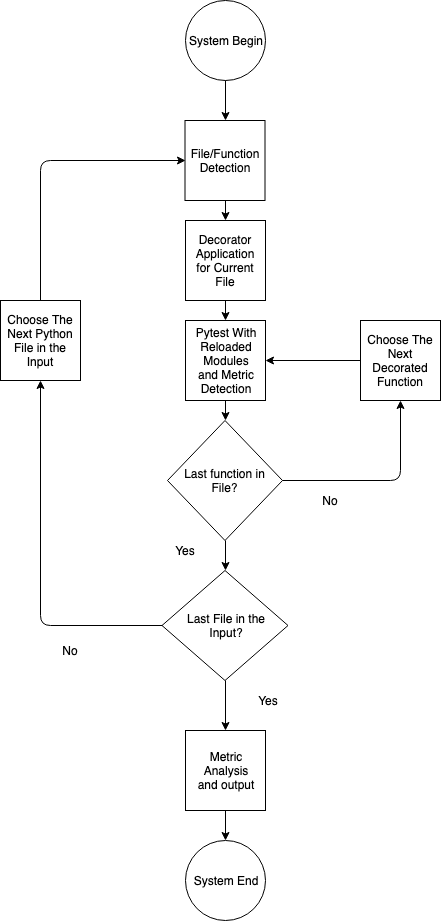
\includegraphics[scale = .6]{images/flow.png}
    \caption{System flow of Function-Fiasco}~\label{systemFlow}
  \end{figure}


% TODO functionality has changed so that the test files are no longer being observed.
  \subsection{System Collection}
    % * System Detection
      The system collection is a process that gives Function-Fiasco the knowledge of what files are being used in the system and the number of functions in each. This process is crucial because it is how Function-Fiasco knows when each file has been analyzed and so it can create a fully examined list of the functions in the system.

    %   * User provided
          Function-Fiasco begins with the user providing the path to the system that the user would like to analyze for pseudo-tested methods. This information is crucial as it provides the location of the root directory of the system and the location of the source code or files. This is accomplished by providing Function-Fiasco a command line argument when starting the system. An example would be \texttt{python3 functionfiasco.py ../fake/ src}.
    %   * Recursive File Exploration
          Once the file path is provided, the next step for Function-Fiasco is file exploration. Since software systems are very complex and could vary in their configuration, Function-Fiasco recursively searches through all paths of the system to find any Python files. The reason that it is looking for this type of file is so that it finds all source code files. It is important to note that test files are ignored from this search. This whole phase can be represented in Figure \ref{systemFlow} as the system begin bubble and the File/Function Detection block. This is because after a new file has been detected, the function detection begins. The function detection process uses AST to search for an AST object called a FunctionDef. This object provides the ability to use the name of the function as it helps to provide the list of associated tests that are pseudo-testing the function. The function detection then provides the number of functions found in each file to give Function-Fiasco the capability of calculating the function coverage for the system. After the functions have been determined in each file, the next step is to begin the analysis for the file that is under scrutiny. This begins with the function and method decoration for that file.

  \subsection{Method Decoration}
  % * File Decoration
    The file decoration phase is one of the most imporant for the execution of Function-Fiasco. This is because Function-Fiasco is using the process for mutation testing and therefore needed a way to analyze a system without altering the source code in a major way. The decoration use in Python was chosen as it is not as intrusive as completely changing the function to eliminate the functionality from it. In fact it provides the ability to maintain the type output that the function would normally have. This type of analysis would allow the testing for other types of ``pseudo-testedness,'' other than the arbitrary check of if the test passes with completely swallowed functionality.

  %   * Per file basis
        The decorator is applied on per file basis. This is in part because of the file exploration. Since Function-Fiasco is using recursive file search to locate all source files, it is helpful to run the analysis on a per file basis to eliminate the number of iterations for the system. It would be unnecessary for Function-Fiasco to find all of the files, then iterate again to add the decorator. On a large system, this process of the double iteration can very quickly become computationally expensive. Another line that is added to each file that allows the decorator to work properly. The line is simply ``\texttt{\textbackslash n \textbackslash n from decorators import skipper \textbackslash n}.'' Without it though, Function-Fiasco would be unable to use the decorator and the system would crash because the applied decorator, \texttt{@skipper}, would be unrecognized.

  %   * All methods receive the decorator
        All functions in the file are decorated at the same time. Function-Fiasco performs one iteration of the file and applies the \texttt{@skipper} decorator call right above every function that is found. This syntax, which can be found in Listing \ref{decoratorExample}, matches the correct usage allowed by Python. Function-Fiasco also has to match the correct spacing of the function that it is being applied to. This is because of the decorators indentation level, the system will crash because it is incorrect usage of the decorator. The reason that they are applied in such a manner is the same as why this is accomplished on the per file basis. The process of adding the decorator, cleaning the file to remove the decorator, and adding it again to the next function would be unnecessarily expensive for the system. Instead Function-Fiasco puts all of the decorators on at the same time and relies on the decorator itself to know if it should apply the manipulation to the file or not.

  %   * Decorator knows what method it should be analyzing
        The decorator is able to accomplish this because functionality has been implemented so that Function-Fiasco knows if the function that is trying to be executed is the file that is currently under scrutiny. Since all tests that are associated with a certain function are executed during the analysis phase it is imporant that any function that is also associated maintains its functionality. So even if 10 methods were executed during the analysis phase, 9 of them would maintain their functionality and the one that does not is masked by the decorator. This is accomplished by adding the name of the function that is currently under scrutiny to the decorator class itself. Since every function is calling to this decorator, the name of all of them is being compared. The only way that the functionality masking and type fuzzing occurs is if the name of the function that is under scrutiny matches the name of the function that is currently being logically determined by the decorator.

  \subsection{Execution and Analysis}
  % * Execution
      The execution phase is where different tests in the test suite of the system are being executed in accordance with the method that is currently under scrutiny. The decorator is meant to do much of the work during the execution, so on the side of Function-Fiasco, there is not much that it needs to do. Function-Fiasco simply runs Pytest in coordination with the aforementioned plugins: PytestFinder and PytestReload. Function-Fiasco provides the method name to PytestFinder and the test suite runs so that only the tests that are associated with the method are executed. This was to cut down on the run time that performing this type of operation can induce. The test suite runs as if the test names were provided. The true execution is performed by the decorator. Since the decorator knows what the correct function to manipulate is, it will allow all other functions to operate as normal but the function that is under scrutiny will have its functionality masked and the return will be fuzzed. After Pytest ends its execution, Function-Fiasco changes the decorator so that the name of the function that was just under scrutiny is forgotten. The analysis is then begun.

  %   * Pytest is run in coordination with PytestFinder and PytestReload
  %   * Method name is given to PytestFinder to reduce the number of tests run
  %   * PER METHOD

  % * Analysis
  %   * Pseudo-tested method data collection
        The analysis begins by collecting the Pytest ouptut from the execution. While Pytest is running, the results of Pytest are being written to a report file so that the results can be examined closer. An example of this report file can be found in Listing \ref{resultOutput}. In this example the output includes which methods were used during the test execution. This information allows Function-fiasco to update the number of used functions so that the coverage may be accurately calculated. The next piece of important information is the test status of \texttt{PASSED}. Function-Fiasco looks for this keyword so that it may update the number of pseudo-tested methods. If this keyword appears on one of the tests, the function is considered pseudo-tested because at least one of the tests is pseudo-testing it. The test name would also be updated to a dictionary entry that contains the name of the function and all of the tests that need to be optimized. This analysis is completed for every function and the results of each are collected and compiled to form an overall assessment of the system and its test suite.

        \begin{figure}[t!]
        \begin{lstlisting}[language = Python, numbers = left, frame = single, caption = Execution of pytestFinder., label = resultOutput]
        ======== test session starts ========
        platform darwin -- Python 3.7.0, Pytest-3.8.0, py-1.6.0, pluggy-0.7.1 -- /usr/local/opt/python/bin/python3.7
        cachedir: .Pytest_cache
        rootdir: /Users/nick/Computer_Science/Function-Fiasco/ffiasco-git, inifile:
        collecting ...

        Methods executed during testing
        #######################
        tester
        #######################
        collected 6 items

        ../fake/tests/test_fake.py::test_tester PASSED [100%]

        ======== 1 passed, 5 warnings in 0.03 seconds ========
        \end{lstlisting}
        \end{figure}


  %   * Update to the number of pseudo-tested methods
  %   * Inclusion of poor tests to the method name
  %   * Repeat of the whole process per file

  \subsection{Results}
  % * Table Creation
      The results phase is based around creating a readable table that developers and testers can use to understand where their system is lacking in terms of testing. It is meant to reflect how the system was operating before Function-Fiasco was run, and what the true behavior is after Function-Fiasco makes observations about the behavior of the system and its test cases.

  %   * Coverage creation
        The first step that Function-Fiasco takes to create the table is to calculate the function coverage of the system. This is accomplished by taking the number of methods that were tested during the execution of the test suite and dividing it by the number of methods. The purpose of this is to allow the user to make a comparison to what amount of the system is believed to be adequately tested. The calcluation is represented as follows:

        \begin{quote}
        \textbf{\textit{Defintion:}} A method \textit{m} $\in$ a program \textit{P} is said to be covered if there exists at least
        one test case \textit{t} $\in$ in \textit{TS}, the test suite of program \textit{P} that triggers the execution of at least one path of the
        body of \textit{m}. \textit{TS} is the test suite of \textit{P}~\cite{vera2017comprehensive}.

        Where (\textbf{\textit{TM}}) is the number of tested methods in \textit{P},

        \begin{equation}
        Coverage = \frac{TM}{NUMM}
        \end{equation}
        \end{quote}

  %   * Collection of the overall number of methods in the system
        The number of overall methods in the system is used as an indicator for the user. It is meant to assist in the explanation of the other metrics, as the user will understand how these numbers are being calculated. The number of methods is collected during the execution of system and is provided to the results phase.

        \begin{quote}
        \textbf{\textit{Defintion:}} The number of methods (\textbf{\textit{NUMM}}) to be produced is representative of the total number of methods in program \textit{P}.
        \end{quote}

  %   * Collection of the number of tested methods in the system
        The number of tested methods in the system is used to explain the coverage of the system. This number is collected during the results of the Pytest run. PytestFinder returns all methods that are used in the test execution, Function-Fiasco collects the names and uses a set for storage to ensure that no functions are double counted.

        \begin{quote}
        \textbf{\textit{Defintion:}} The number of tested methods (\textbf{\textit{NUMTM}}) to be produced is representative of the total number of methods in program \textit{P}.
        \end{quote}

  %   * Collection of the overall number of pseudo-tested methods
        The next step that Function-Fiasco takes is the collection of the overall number of pseudo-tested methods. This number is taken from the dictionary that contains all of the methods and their associated tests that need optimization. This list is comprised during the analysis phase, and it contains the complete list of all of the methods. This is because the results phase occurs after execution and analysis phase, so the list is complete. The length of the list, specifically the amount of keys which comprise the method and tests relationship, is the total number of pseudo-tested methods. Methods that are considered to be not pseudo-tested are not added to this list.

  %   * Create the number of the "truly" tested methods
        After the number of pseudo-tested methods has been collected, the calculation for the number of ``truly'' tested methods can be calculated. This metric is representative of the number of methods in the system that are not being pseudo-tested, but are still being adequately tested by the system. The calculation is as follows:

        \begin{quote}
        \textbf{\textit{Defintion:}} The number of truly-tested methods (\textbf{\textit{NUMTTM}}) to be produced is representative of the total number of adequately tested methods in program \textit{P}.

        \begin{equation}
        NUMTTM = NUMTM - NUMPTM
        \end{equation}
        \end{quote}

  %   * Actual Coverage Creation
        The updated coverage is the overall result of the execution of Function-Fiasco. It is representative of the function coverage with all that are pseudo-tested removed. The updated coverage shows the fault detection effectiveness of the test suite. The calculation is as follows:
        \begin{quote}
        \begin{equation}
        UC = \frac{NUMTTM}{NUMM}
        \end{equation}
        \end{quote}

  %   * Table is created and shown
        Once all metrics have been created, they are compiled into a table, that is shown to the user. The table when compiled can explain the shortcomings in the test suite that is under scrutiny. It provides all pertinent information that can be used to fully examine the test suite. An example of the table is shown in Listing \ref{tableOutput}. Statement coverage for the system has been included in the table. It is important for the user to be able to compare the metric that they have been using previously with the updated metric.

        \begin{figure}[t!]
        \begin{lstlisting}[language = Python, frame = single, basicstyle=\tiny]
   +-----------+----------+---------+---------+----------+---------------+---------+----------+
   | Statement |          |         | Number  |          |    Number     | Number  |          |
   | Coverage  | Initial  | Number  |   of    | Fiascoed |      of       |   of    | Updated  |
   |           | Function |   of    | Tested  |  Methods | Pseudo-tested |  Truly  | Coverage |
   |           | coverage | Methods | Methods |          |    Methods    | Tested  |          |
   |           |          |         |         |          |               | Methods |          |
   +-----------+----------+---------+---------+----------+---------------+---------+----------+
   |    67%    |   0.44   |   730   |   319   |    16    |       9       |   310   |   0.42   |
   +-----------+----------+---------+---------+----------+---------------+---------+----------+
        \end{lstlisting}
        \caption{Example of the table output.}~\label{tableOutput}
        \end{figure}

  %   * Option for the tests that need optimization
        The final part of the overall execution is an option to see the tests that need optimization. This is an option mainly because of the potential length for this section. Computer science systems are very complex and may contain a numerous number of functions and tests. Based on the size and complexity, this list could very easily become long and difficult to read.
